\documentclass[11pt]{article}
\usepackage[textwidth=18.0cm, textheight=23.0cm, top=2.0cm]{geometry}
\usepackage{pst-all}
\usepackage{amssymb}
\usepackage{tikz}
\usepackage{underscore}\begin{document}
\pagestyle{empty}


ClassName: \underline{\textbf{Class_03.2bp-11}}
\par
BinSize: \underline{\textbf{40 × 40}}
\par
ReduceSize: \underline{\textbf{40 × 40}}
\par
TypeNum: \underline{\textbf{40}}
\par
Num: \underline{\textbf{40}}
\par
OutS: \underline{\textbf{12800}}
\par
InS: \underline{\textbf{11400}}
\par
Rate: \underline{\textbf{0.891}}
\par
UB: \underline{\textbf{8}}
\par
LB0: \underline{\textbf{8}}
\par
LB: \underline{\textbf{8}}
\par
LBWithCut: \underline{\textbf{8}}
\par
NodeCut: \underline{\textbf{0}}
\par
ExtendedNodeCnt: \underline{\textbf{1}}
\par
GenNodeCnt: \underline{\textbf{1}}
\par
PrimalNode: \underline{\textbf{0}}
\par
ColumnCount: \underline{\textbf{8}}
\par
TotalCutCount: \underline{\textbf{0}}
\par
RootCutCount: \underline{\textbf{0}}
\par
LPSolverCnt: \underline{\textbf{1}}
\par
PricingSolverCnt: \underline{\textbf{0}}
\par
BranchAndBoundNum: \underline{\textbf{1}}
\par
isOpt: \underline{\textbf{true}}
\par
TimeOnInitSolution: \underline{\textbf{3.670 s}}
\par
TimeOnPrimal: \underline{\textbf{0.000 s}}
\par
TimeOnPricing: \underline{\textbf{0.000 s}}
\par
TimeOnRmp: \underline{\textbf{0.062 s}}
\par
TotalTime: \underline{\textbf{3.795 s}}
\par
\newpage


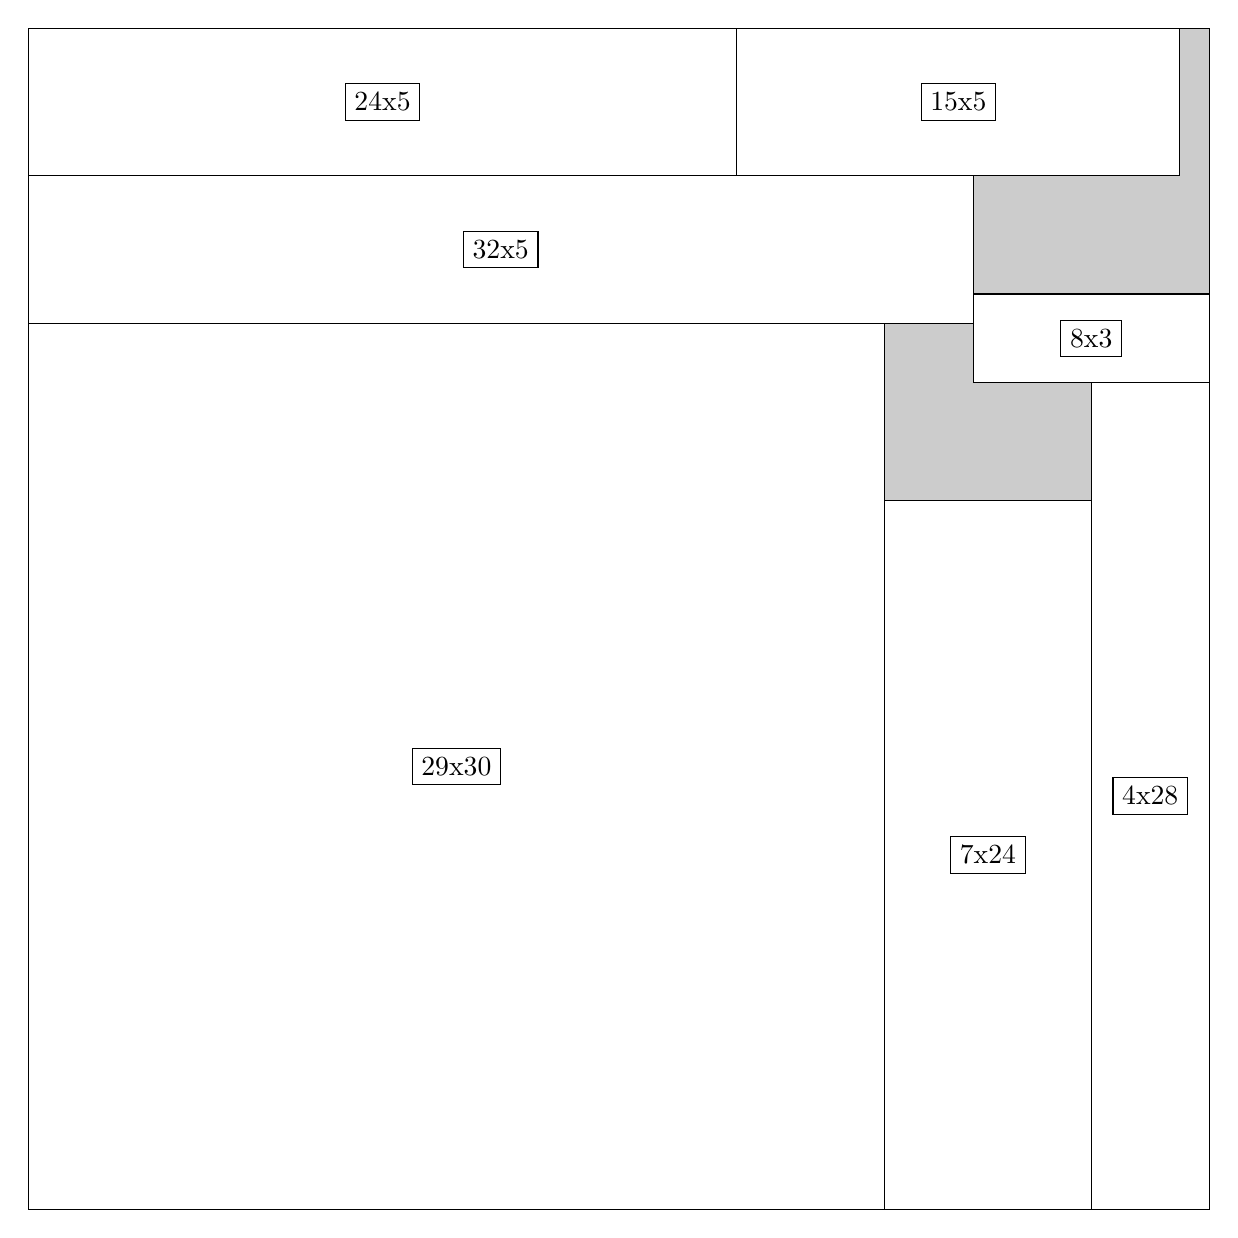
\begin{tikzpicture}[shorten >=1pt,scale=1.0,every node/.style={scale=1.0},->]
\tikzstyle{vertex}=[circle,fill=black!25,minimum size=14pt,inner sep=0pt]
\filldraw[fill=gray!40!white, draw=black] (0,0) rectangle (15.0,15.0);
\foreach \name/\x/\y/\w/\h in {29x30/0.0/0.0/10.875/11.25,7x24/10.875/0.0/2.625/9.0,32x5/0.0/11.25/12.0/1.875,24x5/0.0/13.125/9.0/1.875,4x28/13.5/0.0/1.5/10.5,15x5/9.0/13.125/5.625/1.875,8x3/12.0/10.5/3.0/1.125}
\filldraw[fill=white!40!white, draw=black] (\x,\y) rectangle node[draw] (\name) {\name} ++(\w,\h);
\end{tikzpicture}


w =29 , h =30 , x =0 , y =0 , v =870
\par
w =7 , h =24 , x =29 , y =0 , v =168
\par
w =32 , h =5 , x =0 , y =30 , v =160
\par
w =24 , h =5 , x =0 , y =35 , v =120
\par
w =4 , h =28 , x =36 , y =0 , v =112
\par
w =15 , h =5 , x =24 , y =35 , v =75
\par
w =8 , h =3 , x =32 , y =28 , v =24
\par
\newpage


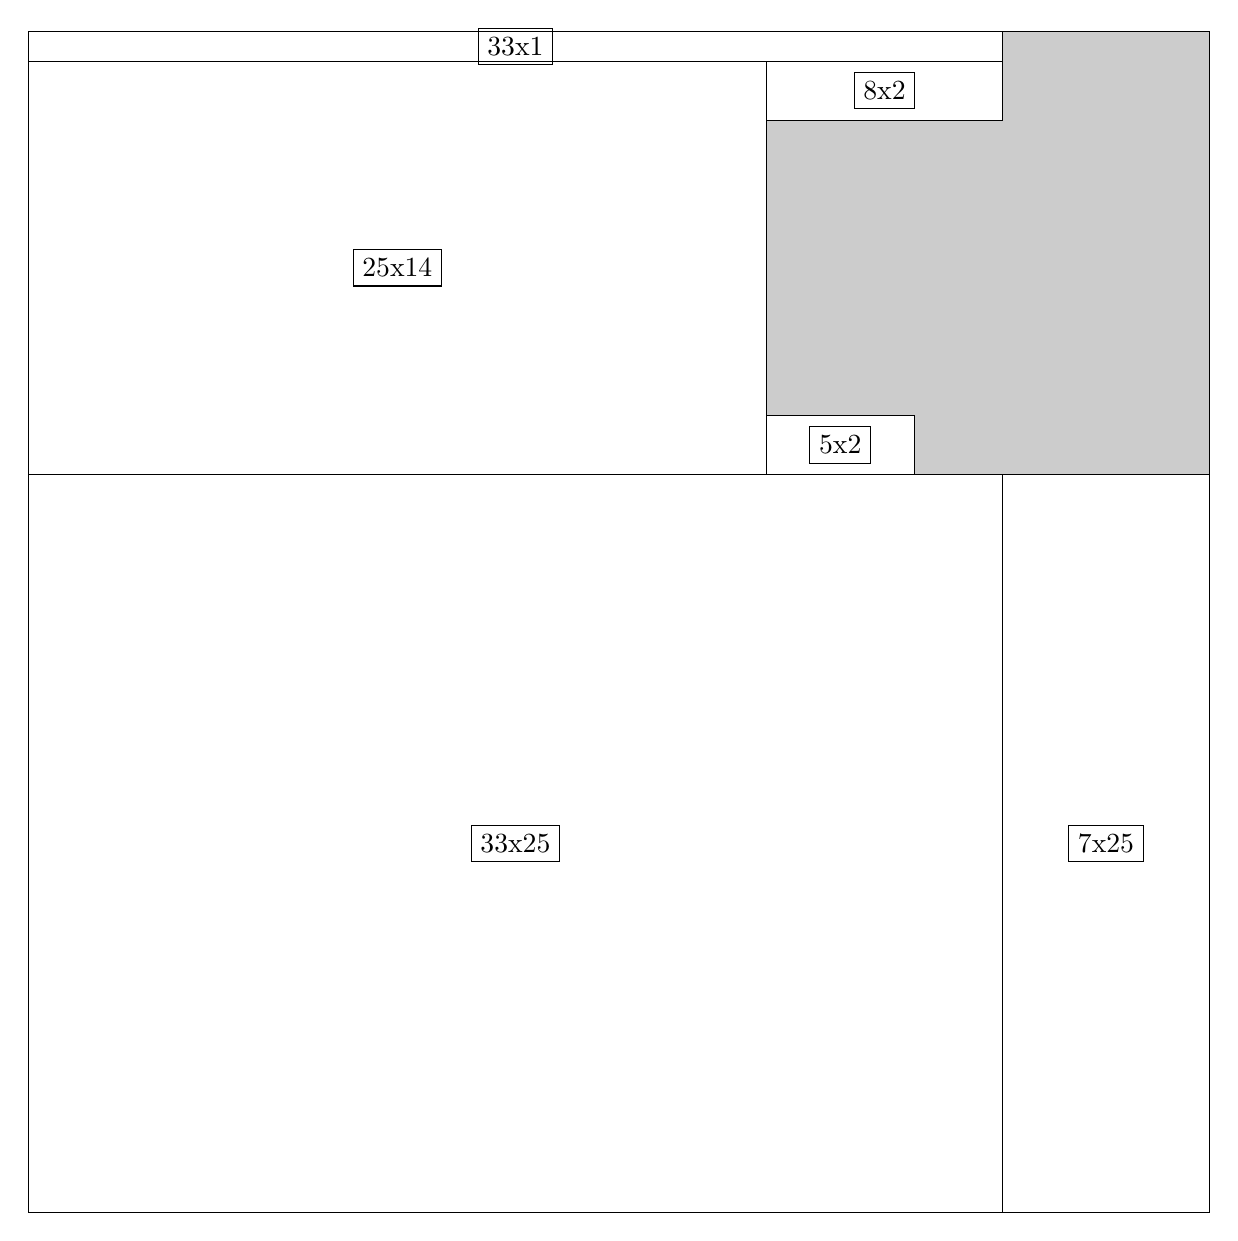
\begin{tikzpicture}[shorten >=1pt,scale=1.0,every node/.style={scale=1.0},->]
\tikzstyle{vertex}=[circle,fill=black!25,minimum size=14pt,inner sep=0pt]
\filldraw[fill=gray!40!white, draw=black] (0,0) rectangle (15.0,15.0);
\foreach \name/\x/\y/\w/\h in {33x25/0.0/0.0/12.375/9.375,25x14/0.0/9.375/9.375/5.25,7x25/12.375/0.0/2.625/9.375,33x1/0.0/14.625/12.375/0.375,8x2/9.375/13.875/3.0/0.75,5x2/9.375/9.375/1.875/0.75}
\filldraw[fill=white!40!white, draw=black] (\x,\y) rectangle node[draw] (\name) {\name} ++(\w,\h);
\end{tikzpicture}


w =33 , h =25 , x =0 , y =0 , v =825
\par
w =25 , h =14 , x =0 , y =25 , v =350
\par
w =7 , h =25 , x =33 , y =0 , v =175
\par
w =33 , h =1 , x =0 , y =39 , v =33
\par
w =8 , h =2 , x =25 , y =37 , v =16
\par
w =5 , h =2 , x =25 , y =25 , v =10
\par
\newpage


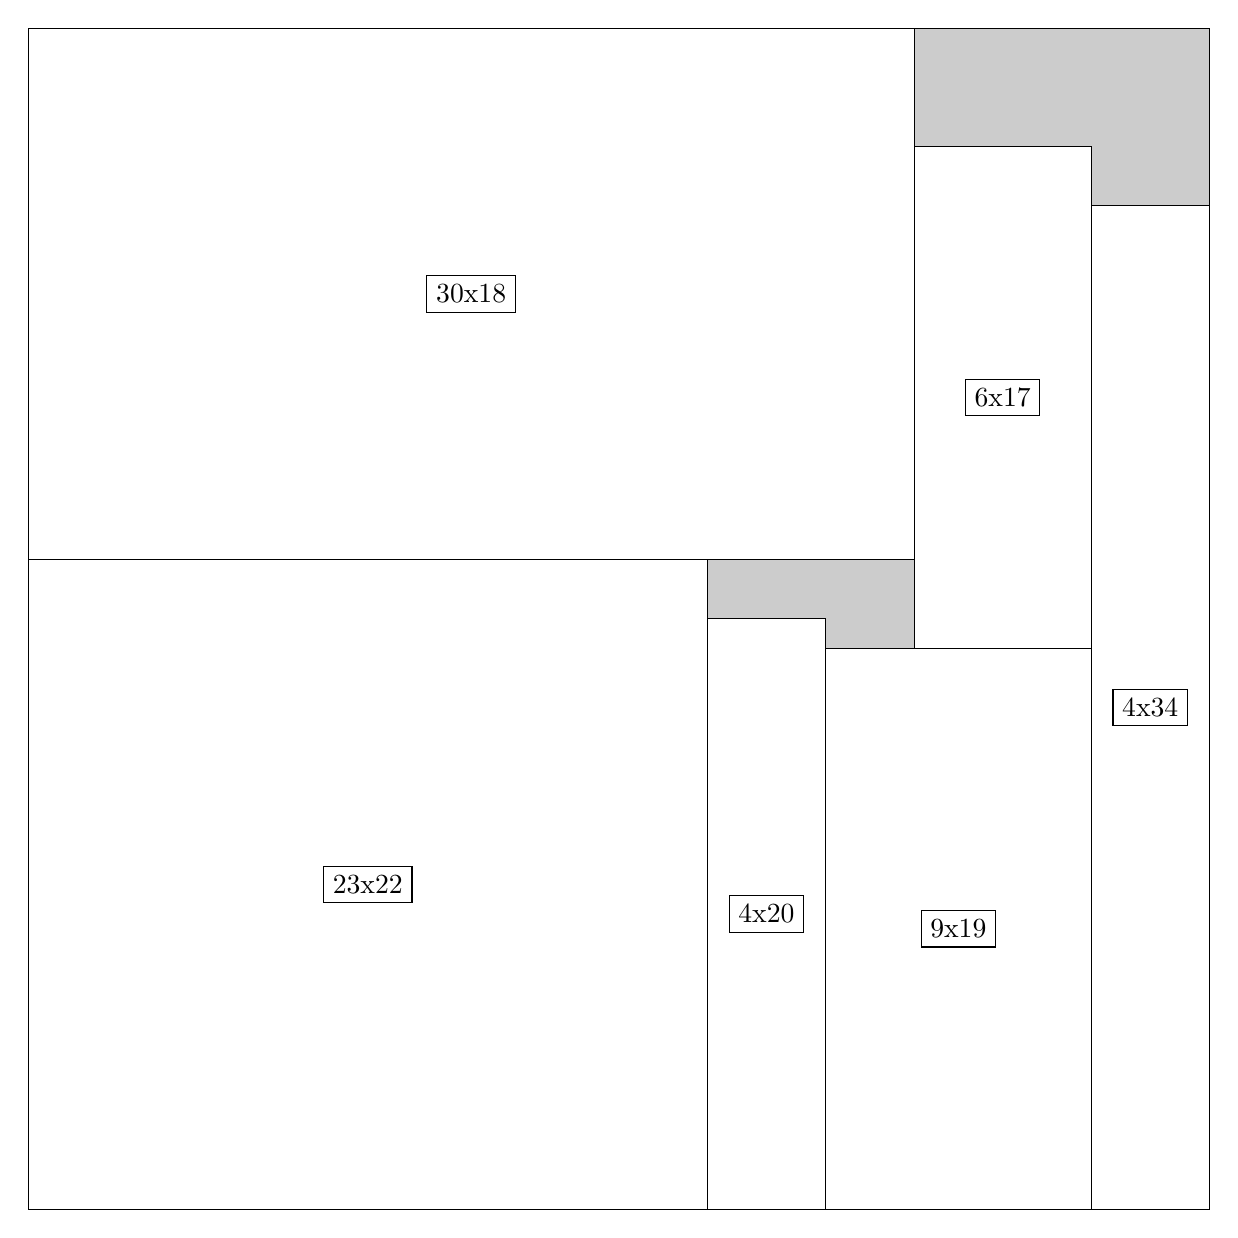
\begin{tikzpicture}[shorten >=1pt,scale=1.0,every node/.style={scale=1.0},->]
\tikzstyle{vertex}=[circle,fill=black!25,minimum size=14pt,inner sep=0pt]
\filldraw[fill=gray!40!white, draw=black] (0,0) rectangle (15.0,15.0);
\foreach \name/\x/\y/\w/\h in {4x20/8.625/0.0/1.5/7.5,30x18/0.0/8.25/11.25/6.75,9x19/10.125/0.0/3.375/7.125,4x34/13.5/0.0/1.5/12.75,6x17/11.25/7.125/2.25/6.375,23x22/0.0/0.0/8.625/8.25}
\filldraw[fill=white!40!white, draw=black] (\x,\y) rectangle node[draw] (\name) {\name} ++(\w,\h);
\end{tikzpicture}


w =4 , h =20 , x =23 , y =0 , v =80
\par
w =30 , h =18 , x =0 , y =22 , v =540
\par
w =9 , h =19 , x =27 , y =0 , v =171
\par
w =4 , h =34 , x =36 , y =0 , v =136
\par
w =6 , h =17 , x =30 , y =19 , v =102
\par
w =23 , h =22 , x =0 , y =0 , v =506
\par
\newpage


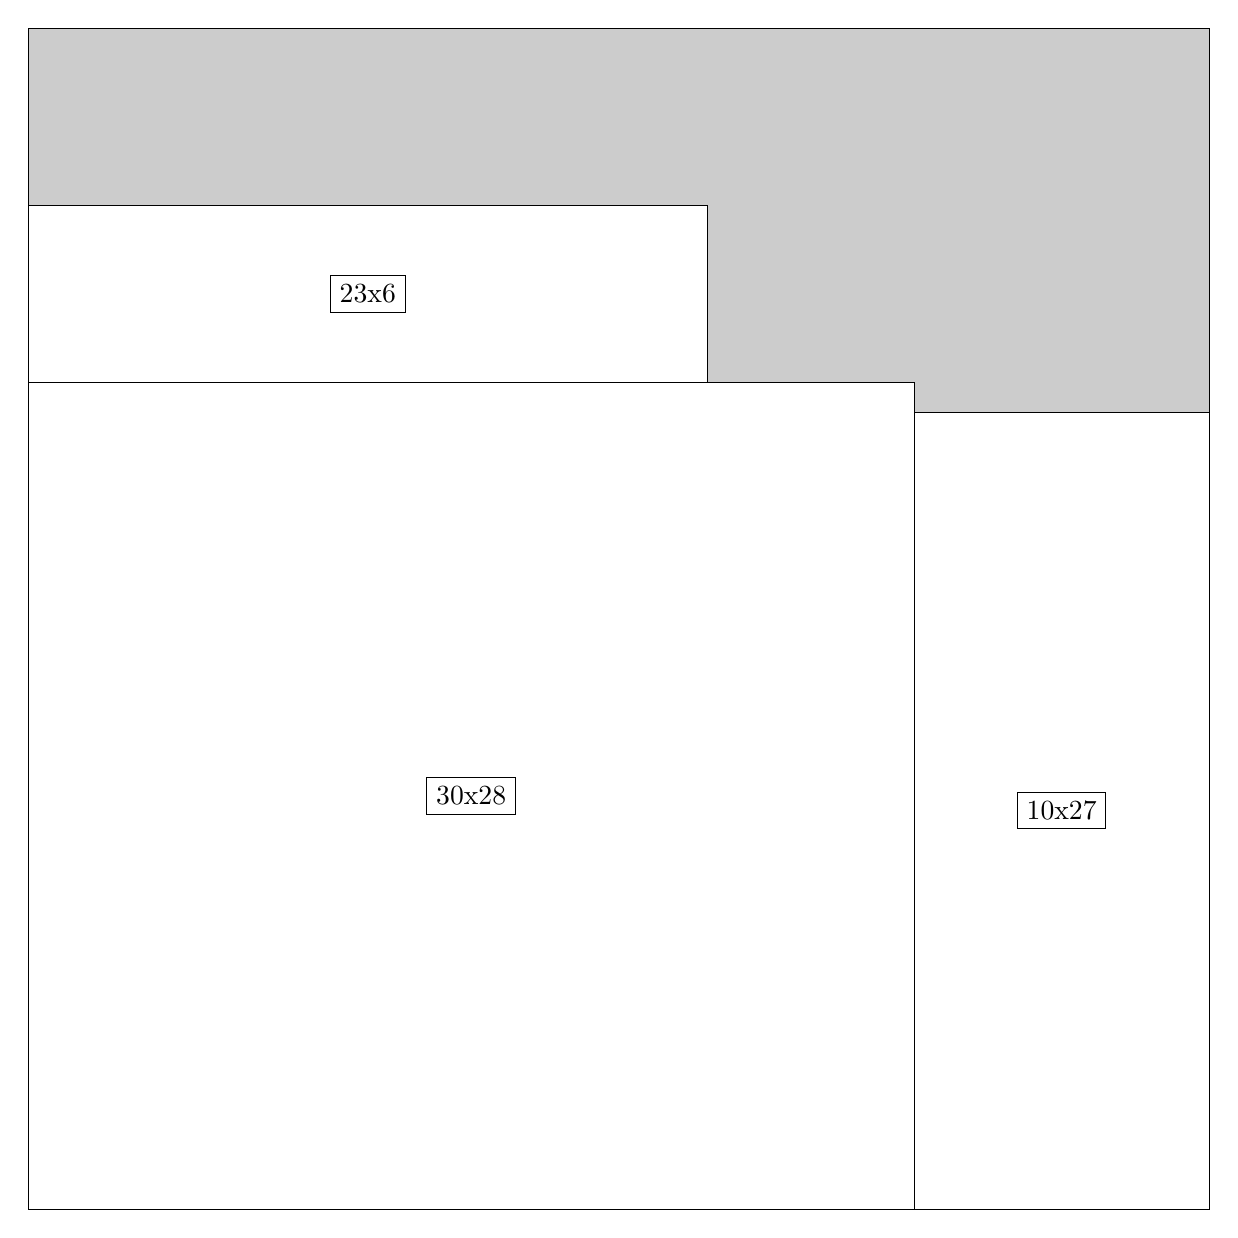
\begin{tikzpicture}[shorten >=1pt,scale=1.0,every node/.style={scale=1.0},->]
\tikzstyle{vertex}=[circle,fill=black!25,minimum size=14pt,inner sep=0pt]
\filldraw[fill=gray!40!white, draw=black] (0,0) rectangle (15.0,15.0);
\foreach \name/\x/\y/\w/\h in {30x28/0.0/0.0/11.25/10.5,10x27/11.25/0.0/3.75/10.125,23x6/0.0/10.5/8.625/2.25}
\filldraw[fill=white!40!white, draw=black] (\x,\y) rectangle node[draw] (\name) {\name} ++(\w,\h);
\end{tikzpicture}


w =30 , h =28 , x =0 , y =0 , v =840
\par
w =10 , h =27 , x =30 , y =0 , v =270
\par
w =23 , h =6 , x =0 , y =28 , v =138
\par
\newpage


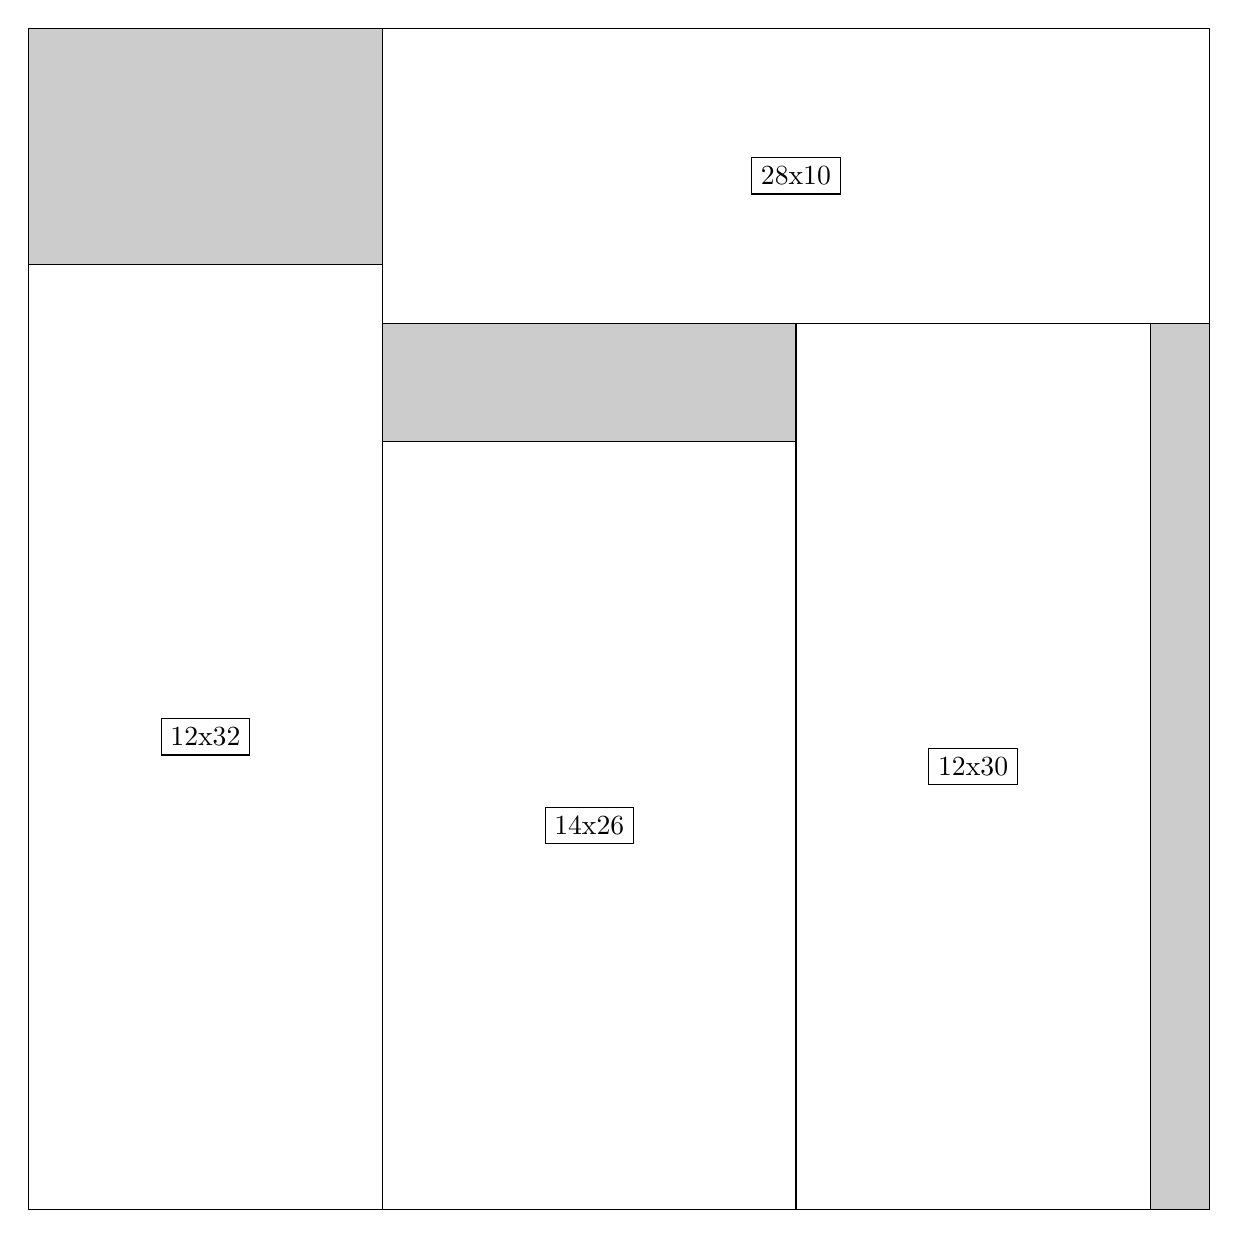
\begin{tikzpicture}[shorten >=1pt,scale=1.0,every node/.style={scale=1.0},->]
\tikzstyle{vertex}=[circle,fill=black!25,minimum size=14pt,inner sep=0pt]
\filldraw[fill=gray!40!white, draw=black] (0,0) rectangle (15.0,15.0);
\foreach \name/\x/\y/\w/\h in {12x32/0.0/0.0/4.5/12.0,14x26/4.5/0.0/5.25/9.75,12x30/9.75/0.0/4.5/11.25,28x10/4.5/11.25/10.5/3.75}
\filldraw[fill=white!40!white, draw=black] (\x,\y) rectangle node[draw] (\name) {\name} ++(\w,\h);
\end{tikzpicture}


w =12 , h =32 , x =0 , y =0 , v =384
\par
w =14 , h =26 , x =12 , y =0 , v =364
\par
w =12 , h =30 , x =26 , y =0 , v =360
\par
w =28 , h =10 , x =12 , y =30 , v =280
\par
\newpage


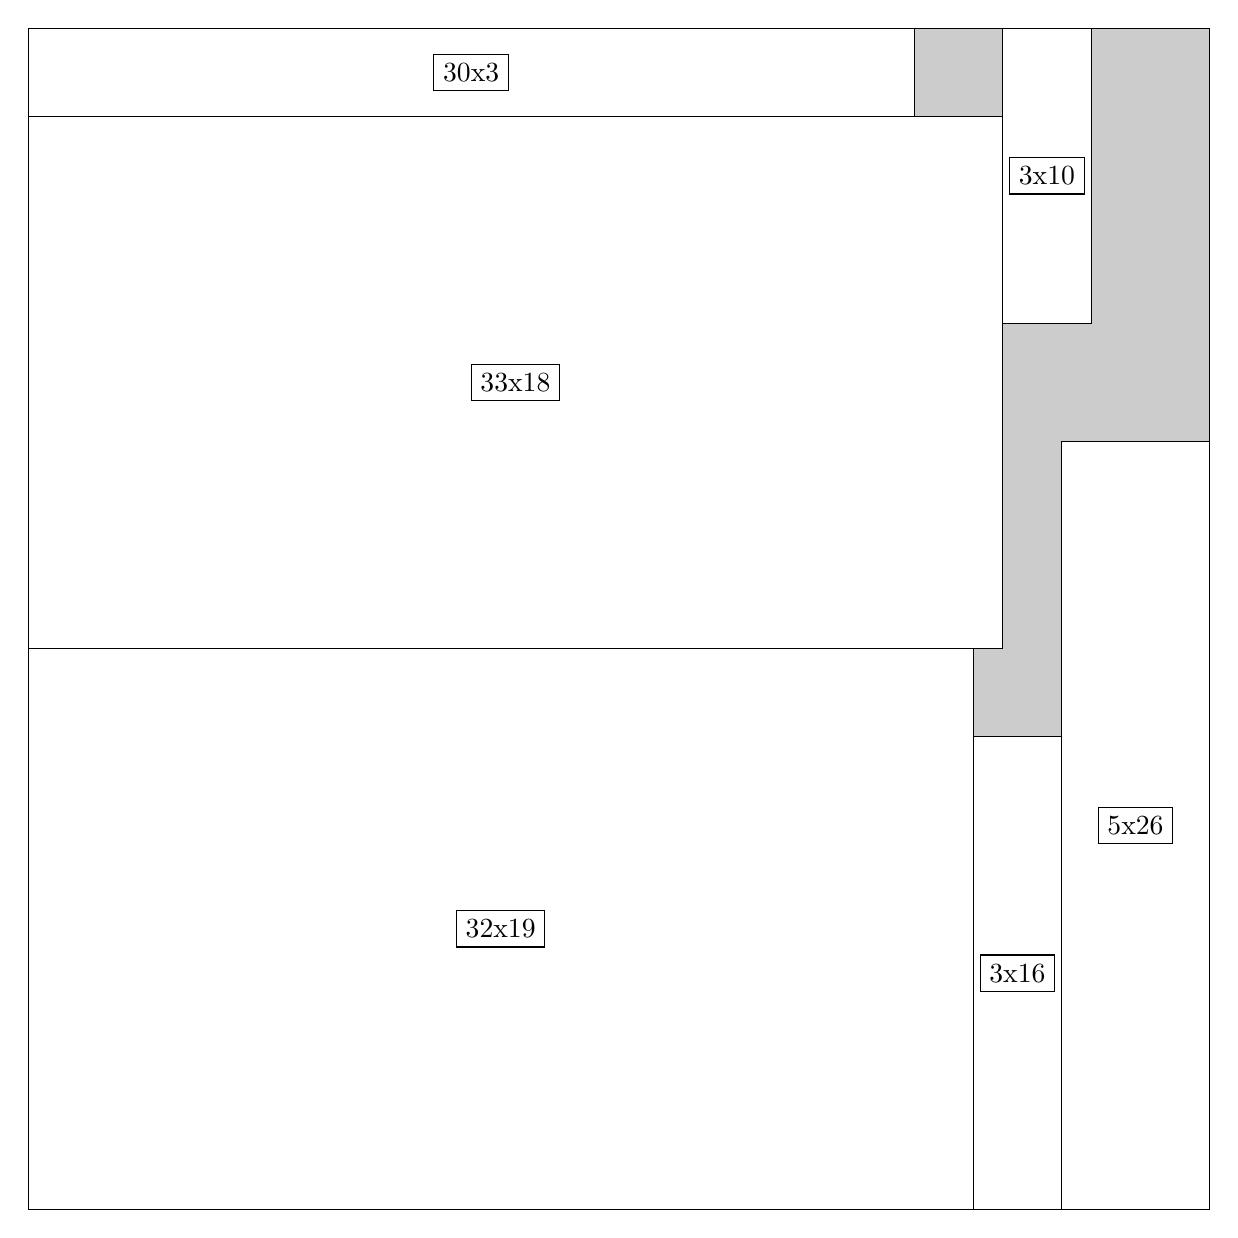
\begin{tikzpicture}[shorten >=1pt,scale=1.0,every node/.style={scale=1.0},->]
\tikzstyle{vertex}=[circle,fill=black!25,minimum size=14pt,inner sep=0pt]
\filldraw[fill=gray!40!white, draw=black] (0,0) rectangle (15.0,15.0);
\foreach \name/\x/\y/\w/\h in {32x19/0.0/0.0/12.0/7.125,33x18/0.0/7.125/12.375/6.75,5x26/13.125/0.0/1.875/9.75,30x3/0.0/13.875/11.25/1.125,3x16/12.0/0.0/1.125/6.0,3x10/12.375/11.25/1.125/3.75}
\filldraw[fill=white!40!white, draw=black] (\x,\y) rectangle node[draw] (\name) {\name} ++(\w,\h);
\end{tikzpicture}


w =32 , h =19 , x =0 , y =0 , v =608
\par
w =33 , h =18 , x =0 , y =19 , v =594
\par
w =5 , h =26 , x =35 , y =0 , v =130
\par
w =30 , h =3 , x =0 , y =37 , v =90
\par
w =3 , h =16 , x =32 , y =0 , v =48
\par
w =3 , h =10 , x =33 , y =30 , v =30
\par
\newpage


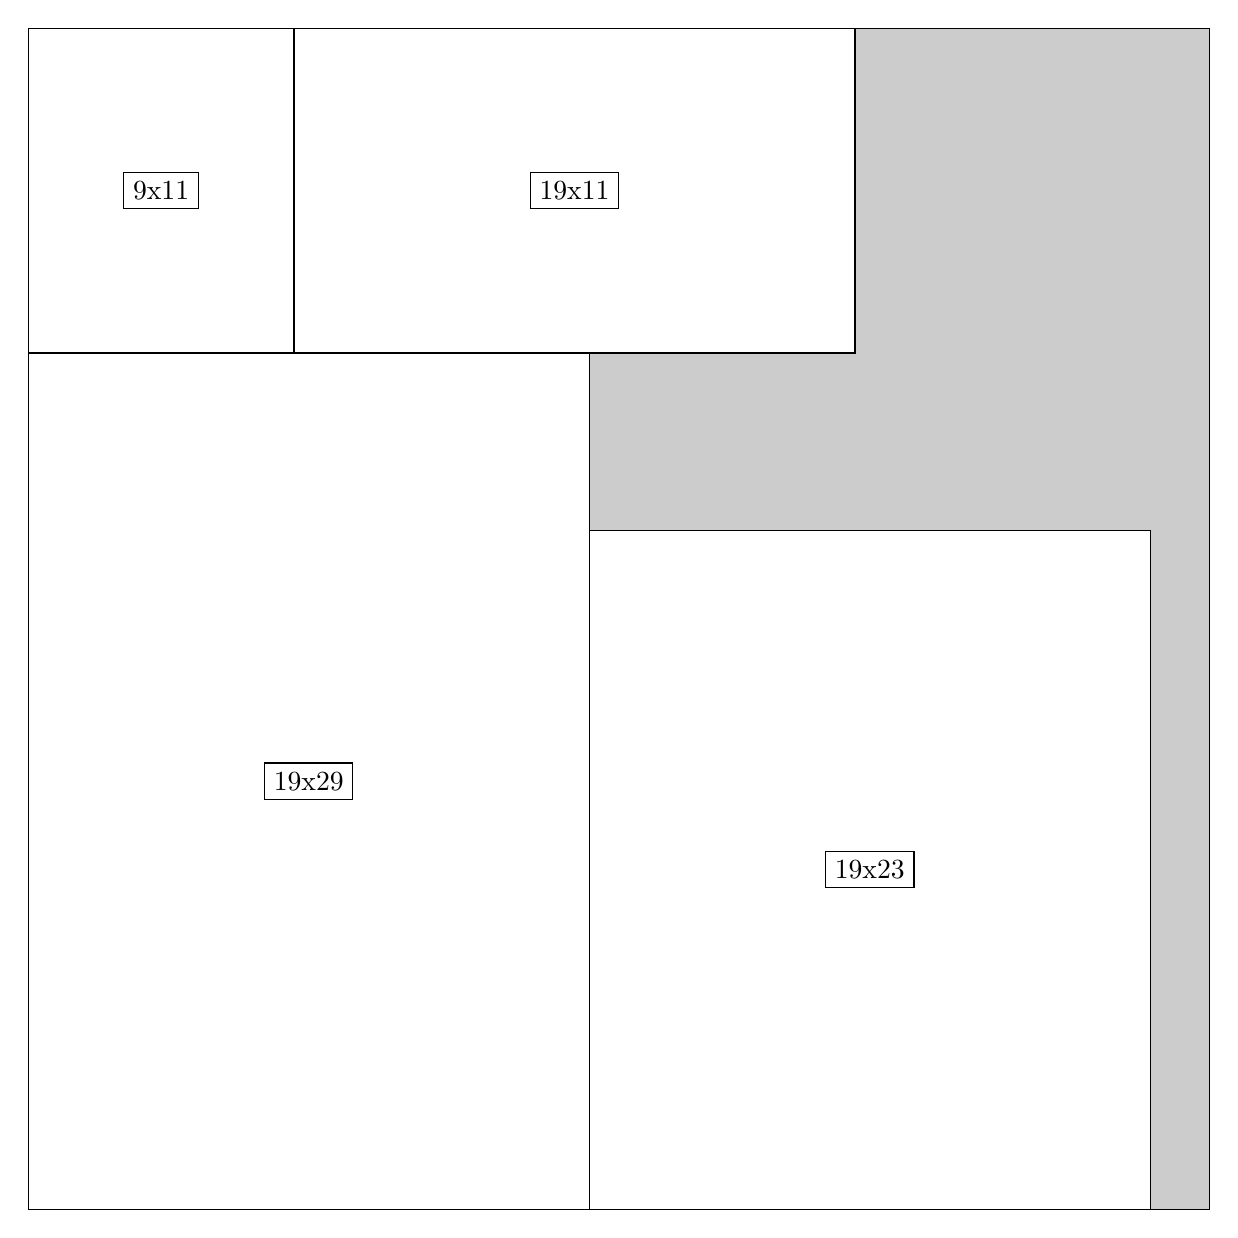
\begin{tikzpicture}[shorten >=1pt,scale=1.0,every node/.style={scale=1.0},->]
\tikzstyle{vertex}=[circle,fill=black!25,minimum size=14pt,inner sep=0pt]
\filldraw[fill=gray!40!white, draw=black] (0,0) rectangle (15.0,15.0);
\foreach \name/\x/\y/\w/\h in {19x29/0.0/0.0/7.125/10.875,9x11/0.0/10.875/3.375/4.125,19x23/7.125/0.0/7.125/8.625,19x11/3.375/10.875/7.125/4.125}
\filldraw[fill=white!40!white, draw=black] (\x,\y) rectangle node[draw] (\name) {\name} ++(\w,\h);
\end{tikzpicture}


w =19 , h =29 , x =0 , y =0 , v =551
\par
w =9 , h =11 , x =0 , y =29 , v =99
\par
w =19 , h =23 , x =19 , y =0 , v =437
\par
w =19 , h =11 , x =9 , y =29 , v =209
\par
\newpage


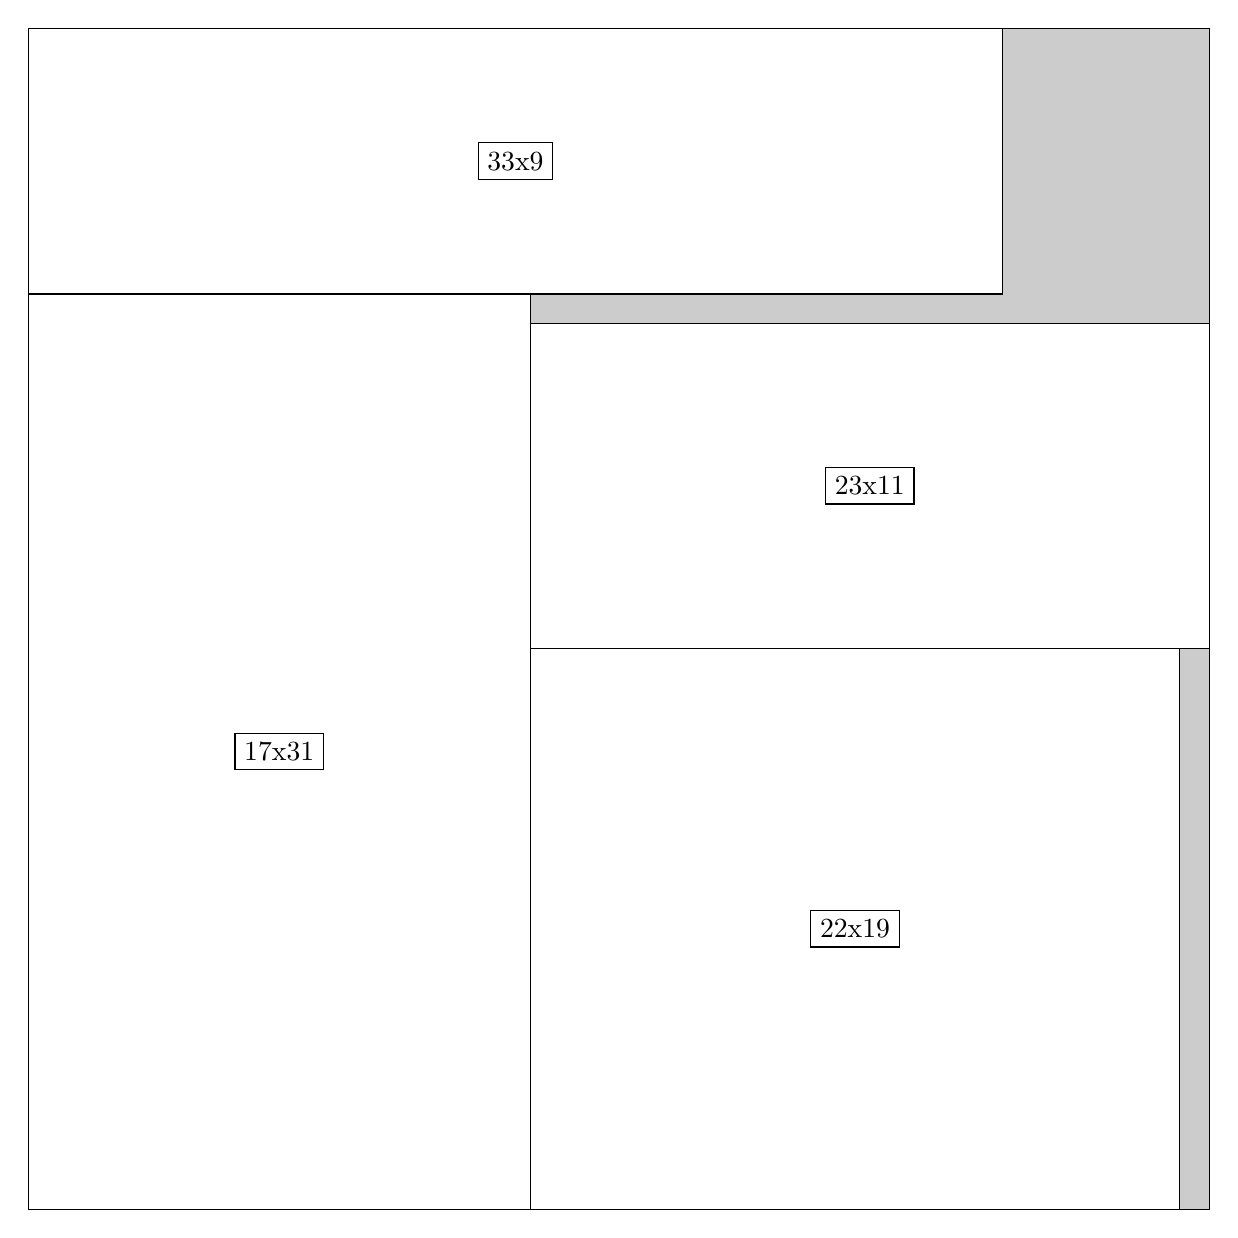
\begin{tikzpicture}[shorten >=1pt,scale=1.0,every node/.style={scale=1.0},->]
\tikzstyle{vertex}=[circle,fill=black!25,minimum size=14pt,inner sep=0pt]
\filldraw[fill=gray!40!white, draw=black] (0,0) rectangle (15.0,15.0);
\foreach \name/\x/\y/\w/\h in {17x31/0.0/0.0/6.375/11.625,22x19/6.375/0.0/8.25/7.125,33x9/0.0/11.625/12.375/3.375,23x11/6.375/7.125/8.625/4.125}
\filldraw[fill=white!40!white, draw=black] (\x,\y) rectangle node[draw] (\name) {\name} ++(\w,\h);
\end{tikzpicture}


w =17 , h =31 , x =0 , y =0 , v =527
\par
w =22 , h =19 , x =17 , y =0 , v =418
\par
w =33 , h =9 , x =0 , y =31 , v =297
\par
w =23 , h =11 , x =17 , y =19 , v =253
\par
\newpage


\end{document}